En este mundo digital en el que vivimos, parte de los elementos más importantes son los credenciales a las diversas \glspl{cuenta} que pueda tener un usuario. Por ello estos credenciales no deberían repetirse ya que constantemente estos credenciales son expuestos al público tras ataques informáticos\cite{pwnedwebs}, sin embargo somos seres humanos, así que desafortunadamente nuestra memoria nos puede fallar, por lo que es surrealista esperar que un usuario recuerde todos los credenciales de sus diversas \glspl{cuenta}. Por ello es recomendable usar un administrador de contraseñas.

Con una \gls{vault} de Bitwarden este problema se soluciona fácilmente. Sin embargo acceder a una \gls{cuenta} no siempre es tan fácil, en concreto cuando se quiere entrar a una \gls{cuenta} en un dispositivo desconocido. Existen 2 formas de lograrlo:
\begin{itemize}
    \item Introducir los credenciales de la \gls{cuenta}, exponiendo entonces a este dispositivo desconocido la clave maestra de la \gls{vault}
    \item Buscar los credenciales en la \gls{vault} y enviarlos por Bitwarden Send, o escribirlos a mano.
\end{itemize}

En el caso de acceder directamente a la \gls{vault} desde el dispositivo objetivo, existen situaciones específicas en las que es imposible o bien poco seguro:
\begin{itemize}
    \item Cuando la clave es el inicio de sesión del propio dispositivo, la forma de desbloquear el mismo, por tanto, aún no se puede tener acceso a la \gls{vault}.
    \item Cuando el dispositivo no posee conexión a internet, por ejemplo, acceder a una base de datos interna de una empresa \textit{on-site}.
    \item Cuando se pone en duda la seguridad del dispositivo. Aunque, por supuesto con \gls{2fa} activada tendríamos una gran protección ante la posibilidad de que alguien con intenciones maliciosas conozca nuestra clave maestra, pero no por ello deberíamos ir pregonando dicha clave, como hizo el actual multimillonario Gabe Newell en 2011. \cite{gabepass}
    \item Cuando el dispositivo objetivo se encuentra bastante limitado, sin permisos de administrador, sin acceso a navegador y/o sin aplicación nativa de Bitwarden. Por ejemplo una consola de videojuegos o una Smart TV.
\end{itemize}

Por otro lado el servicio Bitwarden Send\cite{sendblog} está planteado para \textbf{enviar} datos, información, \textbf{claves} y archivos \textbf{a otras personas}, pero se sigue pudiendo usar personalmente para enviarse a uno mismo una contraseña, como antaño cuando no era popular el almacenamiento online y uno se enviaba un correo electrónico con un archivo porque se había olvidado el pendrive en casa. Aún así crear un Send es un poco rudimentario, pues requiere muchos pasos y el \gls{url} es bastante largo como para escribirlo a mano. \ref{fig:send-link}
\begin{figure}[H]
    \centering
    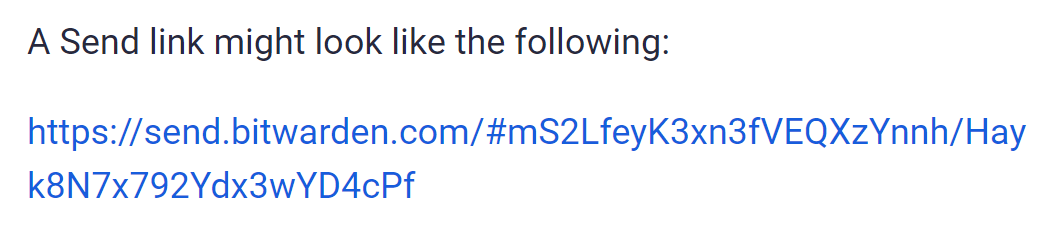
\includegraphics[width=\textwidth]{gfx/send-link.png}
    \caption{Un \gls{url} de Bitwarden Send. \href{https://bitwarden.com/blog/bitwarden-send-how-it-works/}{Realizado por Bitwarden}.}
    \label{fig:send-link}
\end{figure}
Adicionalmente si la estancia de Bitwarden se encuentra en una red local tras una \gls{vpn} o similar en vez de en un dominio público, sólo se podría acceder al enlace si el dispositivo objetivo se encuentra conectado a la misma \gls{vpn}.

Así llegamos a la solución que en este proyecto hemos implementado. Hoy en día, es muy poco probable no llevar un móvil encima, por ello lo cómodo y simple sería que el móvil escribiese por nosotros los credenciales específicos, evitando así exponer la clave maestra. Para llevar a cabo dicha tarea usaremos InputStick como medio de transmisión.